\documentclass[a4paper,11pt]{report}

% =======================================================
% PACKAGES & CONFIGURATION
% =======================================================
\usepackage[utf8]{inputenc}
\usepackage[T1]{fontenc}
\usepackage[english]{babel}
\usepackage{amsmath, amsfonts, amssymb, amsthm}
\usepackage{geometry}
\usepackage{parskip}
\usepackage{fancyhdr}
\usepackage{tcolorbox}
\usepackage{hyperref}
\usepackage{booktabs}
\usepackage{enumitem}

% --- Graphics & Plots ---
\usepackage{pgfplots}
\pgfplotsset{compat=1.18}
\usepackage{tikz}
\usetikzlibrary{patterns}

% --- Layout Settings ---
\geometry{hmargin=2.5cm,vmargin=2.5cm}
\definecolor{exBlue}{RGB}{0, 60, 120}
\definecolor{exRed}{RGB}{180, 40, 40}
\definecolor{exGreen}{RGB}{0, 100, 50}
\definecolor{exPurple}{RGB}{100, 0, 100}

% --- Header/Footer ---
\pagestyle{fancy}
\fancyhead[L]{\textbf{Applied Quantitative Trading}}
\fancyhead[R]{Concrete Scenarios}
\fancyfoot[C]{\thepage}

% =======================================================
% DOCUMENT START
% =======================================================
\begin{document}

% --- TITLE PAGE ---
\begin{titlepage}
    \centering
    \vspace*{2cm}
    {\Huge \textbf{Deep Dive: Trading Strategies}}\\[0.5cm]
    {\Large \textit{Step-by-Step Numerical Examples}}\\[2cm]
    
    \textbf{Module 17 (Extended)}\\[1cm]
    
    \begin{tcolorbox}[colback=gray!10, title=\textbf{Objective}]
    In an interview, do not just define the strategy. Walk the interviewer through a trade lifecycle:
    \begin{enumerate}
        \item Entry Signal (Why do we trade?)
        \item Execution (What do we buy/sell?)
        \item PnL Mechanics (Where does the money come from?)
        \item Exit (When do we leave?)
    \end{enumerate}
    \end{tcolorbox}
    
    \vfill
    {\large \today}
\end{titlepage}

\tableofcontents
\newpage

% =======================================================
% CHAPTER 1: VOLATILITY TRADING (GAMMA SCALPING)
% =======================================================
\chapter{Volatility Trading: Gamma Scalping}

Many candidates know what a Straddle is. Few can explain how to monetize it via \textbf{Gamma Scalping}.

\section{The Concept}
You buy an option (Long Gamma). You hedge it initially to be Delta Neutral.
\begin{itemize}
    \item If the stock goes UP, your Delta increases (becomes positive). To stay neutral, you must SELL shares.
    \item If the stock goes DOWN, your Delta decreases (becomes negative). To stay neutral, you must BUY shares.
\end{itemize}
\textbf{Result:} You are mechanically "Selling High" and "Buying Low". This trading profit offsets the cost of the option (Theta).

\section{Numerical Example}

\begin{tcolorbox}[colback=exBlue!5!white,colframe=exBlue,title=\textbf{Scenario: The Oscillating Stock}]
\textbf{Initial Setup ($t=0$):}
\begin{itemize}
    \item Stock Price $S_0 = \$100$.
    \item We buy 1 ATM Straddle (Call + Put). Total Premium paid = \$4.
    \item Delta is 0. No shares needed initially.
    \item Gamma is 0.10 (For every \$1 move, Delta changes by 0.10).
\end{itemize}

\textbf{Step 1 ($t=1$): Stock rises to \$102.}
\begin{itemize}
    \item New Delta $\approx 0 + (2 \times 0.10) = +0.20$.
    \item We are now "Long 20 shares" equivalent.
    \item \textbf{Action:} Sell 20 shares at \$102 to return to neutral.
    \item \textit{Cash In: \$2,040.}
\end{itemize}

\textbf{Step 2 ($t=2$): Stock crashes back to \$100.}
\begin{itemize}
    \item New Delta returns to 0.
    \item We are currently "Short 20 shares" (from Step 1).
    \item \textbf{Action:} Buy back 20 shares at \$100.
    \item \textit{Cash Out: \$2,000.}
\end{itemize}

\textbf{PnL Result:}
We sold at \$102 and bought at \$100.
Profit = $20 \times (\$102 - \$100) = \mathbf{+\$40}$.
\end{tcolorbox}

\begin{center}
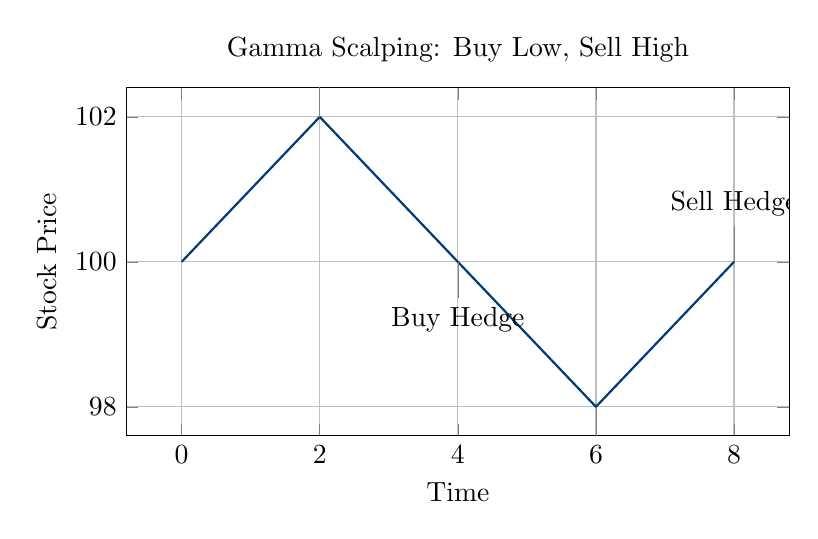
\begin{tikzpicture}
    \begin{axis}[
        width=10cm, height=6cm,
        xlabel={Time}, ylabel={Stock Price},
        title={Gamma Scalping: Buy Low, Sell High},
        ytick={98, 100, 102},
        grid=major
    ]
    \addplot[thick, exBlue] coordinates {(0,100) (2,102) (4,100) (6,98) (8,100)};
    
    \node[coordinate, pin=above:{Sell Hedge}] at (axis cs: 2, 102) {};
    \node[coordinate, pin=below:{Buy Hedge}] at (axis cs: 4, 100) {};
    \node[coordinate, pin=below:{Buy Hedge}] at (axis cs: 6, 98) {};
    \node[coordinate, pin=above:{Sell Hedge}] at (axis cs: 8, 100) {};
    \end{axis}
\end{tikzpicture}
\end{center}

% =======================================================
% CHAPTER 2: STATISTICAL ARBITRAGE (PAIRS)
% =======================================================
\chapter{Stat Arb: Pairs Trading}

\section{The Concept}
We find two stocks, Coke (KO) and Pepsi (PEP), that historically move together. We model the \textbf{Spread}:
$$ S_t = \ln(P_{KO}) - \beta \ln(P_{PEP}) $$
We assume $S_t$ is mean-reverting (Ornstein-Uhlenbeck).

\section{Numerical Example}

\begin{tcolorbox}[colback=exRed!5!white,colframe=exRed,title=\textbf{Scenario: The Divergence}]
\textbf{Parameters:}
\begin{itemize}
    \item Historical Mean of Spread = 0.
    \item Standard Deviation of Spread ($\sigma$) = \$1.00.
    \item Beta $\beta = 1$ (for simplicity).
\end{itemize}

\textbf{Day 1: Market Normal}
\begin{itemize}
    \item KO = \$50, PEP = \$50. Spread = 0. ($Z$-score = 0).
    \item \textbf{Action:} Do nothing.
\end{itemize}

\textbf{Day 2: The Shock (Bad news for PEP)}
\begin{itemize}
    \item KO = \$50, PEP drops to \$47.
    \item Spread = $50 - 47 = +3$.
    \item $Z$-score = $(3 - 0)/1 = +3$ (3 Sigma Event!).
    \item \textbf{Signal:} The spread is too high. It must fall.
    \item \textbf{Action:} Sell the expensive one (KO), Buy the cheap one (PEP).
    \item \textit{Trade:} Short 1 share KO @ \$50, Long 1 share PEP @ \$47.
\end{itemize}

\textbf{Day 3: Convergence (Mean Reversion)}
\begin{itemize}
    \item Market stabilizes. KO drops to \$49, PEP recovers to \$49.
    \item Spread = $49 - 49 = 0$. Target reached.
    \item \textbf{Action:} Close positions.
    \item Buy back KO @ \$49 (Gain \$1). Sell PEP @ \$49 (Gain \$2).
\end{itemize}

\textbf{Total Profit:} $\mathbf{+\$3.00}$. (Risk-free profit if correlation holds).
\end{tcolorbox}

% =======================================================
% CHAPTER 3: MOMENTUM (TREND FOLLOWING)
% =======================================================
\chapter{Momentum Strategies}

\section{The Concept}
"The trend is your friend." We use \textbf{Moving Average Crossovers} to identify trends early. This captures huge moves (like Bitcoin 2017/2020 or Oil shocks) but loses money in choppy sideways markets ("Whipsaw").

\section{Numerical Example}

\begin{tcolorbox}[colback=exPurple!5!white,colframe=exPurple,title=\textbf{Scenario: The Golden Cross}]
\textbf{Indicators:}
\begin{itemize}
    \item Fast Moving Average (MA-10).
    \item Slow Moving Average (MA-50).
\end{itemize}

\textbf{Week 1-3: Choppy Market}
\begin{itemize}
    \item Asset trades between \$100 and \$105.
    \item MA-10 oscillates around MA-50.
    \item \textbf{PnL:} Small losses due to false signals (buying at \$105, selling at \$104).
\end{itemize}

\textbf{Week 4: The Breakout}
\begin{itemize}
    \item Price jumps to \$110.
    \item MA-10 crosses \textbf{above} MA-50.
    \item \textbf{Action:} BUY at \$110.
\end{itemize}

\textbf{Week 5-10: The Trend}
\begin{itemize}
    \item Price rallies to \$150. We hold.
    \item We do not sell even if price drops to \$145, as long as MA-10 > MA-50.
\end{itemize}

\textbf{Week 11: The Reversal}
\begin{itemize}
    \item Price drops to \$135.
    \item MA-10 crosses \textbf{below} MA-50.
    \item \textbf{Action:} SELL at \$135.
\end{itemize}

\textbf{Result:} Profit = \$135 - \$110 = \$25. We missed the top (\$150) and the bottom (\$100), but we captured the "meat" of the move.
\end{tcolorbox}

% =======================================================
% CHAPTER 4: MARKET MAKING (INVENTORY)
% =======================================================
\chapter{Market Making: Inventory Skewing}

\section{The Concept}
A Market Maker (MM) wants to earn the Bid-Ask spread. The danger is **Inventory Risk**: accumulating a position that loses value.
To manage this, the MM **skews** their quotes to force the market to balance their inventory.

\section{Numerical Example (Avellaneda Logic)}

\begin{tcolorbox}[colback=exGreen!5!white,colframe=exGreen,title=\textbf{Scenario: Managing Risk}]
\textbf{State 0: Neutral Inventory}
\begin{itemize}
    \item Fair Price (Mid): \$100.00.
    \item Standard Spread: \$0.10.
    \item \textbf{MM Quote:} Bid \$99.95 | Ask \$100.05.
\end{itemize}

\textbf{Event: A large seller hits our Bid.}
\begin{itemize}
    \item We buy 1,000 shares at \$99.95.
    \item \textbf{Inventory:} Long +1,000 shares.
    \item \textbf{Risk:} If price drops to \$99.00, we lose \$1,000. We need to sell ASAP.
\end{itemize}

\textbf{Action: Skew the Quotes Downward}
We lower our prices to attract buyers (to sell to them) and discourage sellers.
\begin{itemize}
    \item New Mid assumption: \$99.98.
    \item \textbf{New MM Quote:} Bid \$99.93 | Ask \$100.03.
\end{itemize}

\textbf{Consequence:}
\begin{itemize}
    \item Because our Ask (\$100.03) is cheaper than the market average (\$100.05), buyers flock to us.
    \item We sell our 1,000 shares at \$100.03.
    \item \textbf{PnL:} Bought at \$99.95, Sold at \$100.03. Profit = \$0.08/share.
    \item Inventory is back to 0. Risk is neutralized.
\end{itemize}
\end{tcolorbox}

\begin{center}
\begin{tikzpicture}
    \begin{axis}[
        width=12cm, height=6cm,
        xlabel={Time}, ylabel={Price},
        title={Quote Skewing based on Inventory},
        legend pos=east, grid=major
    ]
    % Mid Price
    \addplot[black, dashed, thick] coordinates {(0,100) (10,100)};
    \addlegendentry{Fair Value}
    
    % Bid/Ask Neutral
    \addplot[exGreen, thick] coordinates {(0,100.05) (4,100.05)};
    \addplot[exGreen, thick] coordinates {(0,99.95) (4,99.95)};
    \node at (axis cs: 2, 100.1) {Neutral Quotes};
    
    % Inventory Event at t=4
    \draw[red, thick, ->] (axis cs: 4, 100) -- (axis cs: 4, 101);
    \node[red] at (axis cs: 4, 101.2) {Inventory Increases};
    
    % Bid/Ask Skewed Down
    \addplot[exRed, ultra thick] coordinates {(4,100.03) (10,100.03)};
    \addplot[exRed, ultra thick] coordinates {(4,99.93) (10,99.93)};
    \node[exRed] at (axis cs: 7, 100.15) {Skewed Quotes (Lower)};
    
    \end{axis}
\end{tikzpicture}
\end{center}

\end{document}